\section{负曲率的检测}
\label{sec:saddle-detection}

梯度已经很小时，怎样判断Hessian还有没有足够负的方向？变量很多时存不下Hessian，所以我们特别关心只用Hessian向量积能走多远，以及找到方向和没找到方向分别说明了什么。

\paragraph{要找的是什么}
对单位向量$\bm{v}$，Rayleigh商$R(\bm{v})=\bm{v}^\top\bm{H}\bm{v}$就是目标沿$\bm{v}$的曲率。谱分解$\bm{H}=\sum_i\lambda_i\bm{q}_i\bm{q}_i^\top$（特征值$\lambda_1\leq\cdots\leq\lambda_n$）给出
\begin{equation}
 \min_{\lVert\bm{v}\rVert_2=1}R(\bm{v})=\lambda_1=\lambda_{\min}(\bm{H}),
 \label{eq:saddle-rayleigh}
\end{equation}
最小值在$\bm{q}_1$处取到。

我们并不需要真的求出$\bm{q}_1$。只要有一个单位向量使$R(\bm{v})\leq-\gamma$，其中$\gamma>0$，它就是负曲率方向，后面的下降分析用到的只是这个不等式。本章的$\gamma$始终表示负曲率的大小。

在原点，$\bm{H}=\operatorname{diag}(-1,1)$，取$\bm{v}=(\cos\theta,\sin\theta)$，Rayleigh商是
\[
 R(\bm{v})=-\cos^2\theta+\sin^2\theta=-\cos2\theta.
\]
夹角在$45^\circ$以内的方向全都是负曲率方向，夹角在$30^\circ$以内的方向满足$R\leq-1/2$。图~\ref{fig:saddle-curvature-cone}显示负曲率方向占据一整个锥，这是检测能够用粗糙办法完成的原因。

\begin{BookInlineFigure}
  \centering
  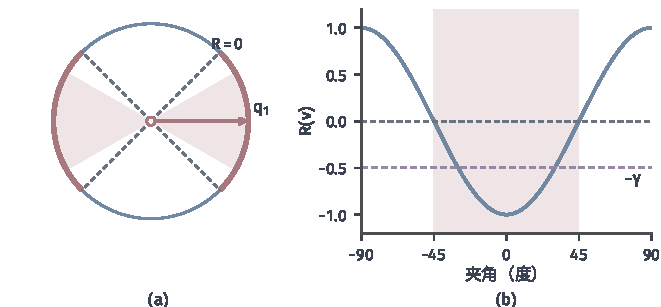
\includegraphics[width=112mm]{figures/05-optimization/02-smooth-optimization/matplotlib/saddle-curvature-cone/figure.pdf}
  \caption{$\bm{H}=\operatorname{diag}(-1,1)$的曲率随方向的变化。(a)单位圆上的红色弧是$R<0$的方向，浅红扇形是$R\leq-1/2$的方向，$\bm{q}_1$是最小特征向量。(b)$R$随方向与$\bm{q}_1$夹角的变化，浅红带是负曲率的范围，紫色虚线是阈值$-\gamma=-1/2$。}
  \label{fig:saddle-curvature-cone}
\end{BookInlineFigure}

\paragraph{矩阵存得下时}
$n$不大时，可以直接计算$\bm{H}$的特征分解，得到$\lambda_{\min}$和$\bm{q}_1$，运算量是$O(n^3)$。如果只需要回答“$\lambda_{\min}$是否大于$-\gamma$”，对$\bm{H}+\gamma\bm{I}$作Cholesky分解更省：分解成功当且仅当$\bm{H}+\gamma\bm{I}$正定，也就是$\lambda_{\min}>-\gamma$。

例中在原点取$\gamma=\tfrac12$，要分解的矩阵是
\[
 \bm{H}+\gamma\bm{I}=\operatorname{diag}\bigl(-\tfrac12,\tfrac32\bigr).
\]
第一个主元就是负的，分解失败，所以$\lambda_{\min}\leq-\tfrac12$。这种方法没有舍入以外的误差，结论是确定的，代价是要存下并分解整个矩阵。

\paragraph{矩阵存不下时}
第~\ref{chap:second-order-methods}章介绍过Hessian向量积，一次乘积的成本与一次梯度同量级。用自动微分可以精确得到它，用差分则只需要两次梯度：
\begin{equation}
 \hat{\bm{u}}=\frac{\nabla f(\bm{x}+h\bm{v})-\nabla f(\bm{x})}{h}.
 \label{eq:saddle-hvp-difference}
\end{equation}

差分带来的误差要记入账。设$\bm{v}$是单位向量，线段$[\bm{x},\bm{x}+h\bm{v}]$落在Hessian为$M$-Lipschitz的区域内。由微积分基本定理，
\[
 \nabla f(\bm{x}+h\bm{v})-\nabla f(\bm{x})-h\bm{H}\bm{v}
 =\int_0^h\bigl(\nabla^2f(\bm{x}+s\bm{v})-\nabla^2f(\bm{x})\bigr)\bm{v}\,\mathrm{d}s.
\]

被积函数的范数不超过$Ms$，积分得$Mh^2/2$。除以$h$，得到
\begin{equation}
 \lVert\hat{\bm{u}}-\bm{H}\bm{v}\rVert_2\leq\frac{Mh}{2}.
 \label{eq:saddle-hvp-error}
\end{equation}

下面用数据验证。在点$\bm{x}=\bm{0}$处取$\bm{v}=(1,1)/\sqrt2$，$h=0.1$，代入梯度~\eqref{eq:saddle-example-derivatives}，由$\nabla f(\bm{0})=\bm{0}$得到
\[
 \hat{\bm{u}}=\begin{bmatrix}h^2v_1^3-v_1\\v_2\end{bmatrix}
 \approx\begin{bmatrix}-0.7036\\0.7071\end{bmatrix},\qquad
 \bm{H}\bm{v}\approx\begin{bmatrix}-0.7071\\0.7071\end{bmatrix}.
\]
实际误差约为$0.0035$，界~\eqref{eq:saddle-hvp-error}给出$0.3$。原点左右对称，一阶误差项恰好抵消，这里的实际误差因此特别小。

图~\ref{fig:saddle-hvp-difference}换到一般的点$(0.3,0.2)$。$h$较大时误差与$h$成正比，$h$太小时舍入误差占主导，这与第~\ref{chap:second-order-methods}章的说法一致。

\begin{BookInlineFigure}
  \centering
  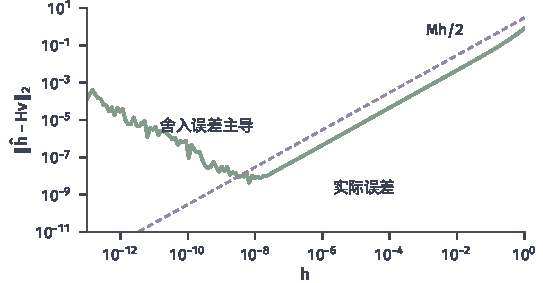
\includegraphics[width=92mm]{figures/05-optimization/02-smooth-optimization/matplotlib/saddle-hvp-difference/figure.pdf}
  \caption{目标~\eqref{eq:saddle-example}在点$(0.3,0.2)$沿$(1,1)/\sqrt2$的差分Hessian向量积误差，绿线是实际误差（双精度计算），紫色虚线是上界$Mh/2$，$M=6$。$h$小于约$10^{-8}$后舍入误差占主导。}
  \label{fig:saddle-hvp-difference}
\end{BookInlineFigure}

\paragraph{主要思想：把最小特征值变成最大特征值}
Hessian向量积最直接的用法是幂迭代：反复乘一个矩阵，向量会转向模最大的特征值所对应的方向。可是我们要的是最小特征值，而$\bm{H}$的最大模特征值可能是最大的正特征值。

解决办法是平移。设$\lVert\bm{H}\rVert_2\leq L$，令
\begin{equation}
 \bm{A}=L\bm{I}-\bm{H}.
 \label{eq:saddle-power-shift}
\end{equation}
$\bm{A}$的特征向量和$\bm{H}$相同，特征值是$a_i=L-\lambda_i\geq0$，最大的$a_1=L-\lambda_{\min}$恰好对应$\bm{H}$的最小特征值。于是对$\bm{A}$作幂迭代：
\begin{equation}
 \bm{v}^{(k+1)}=\frac{\bm{A}\bm{v}^{(k)}}{\lVert\bm{A}\bm{v}^{(k)}\rVert_2},\qquad k=0,1,\ldots
 \label{eq:saddle-power-iteration}
\end{equation}

每轮只用一次Hessian向量积。这里的上标$k$记检测内部的轮数，与外层的迭代$t$区分。把$\bm{v}^{(0)}$按特征向量展开成$\sum_ic_i\bm{q}_i$，$k$轮之后的方向正比于$\sum_ic_ia_i^k\bm{q}_i$，与$a_1$相比较小的分量按几何级数衰减。

这个迭代还有另一层含义。除以$L$之后，$\bm{A}/L=\bm{I}-\tfrac1L\bm{H}$，这正是步长$1/L$的梯度下降在二次目标上的迭代矩阵。所以幂迭代和鞍点附近的梯度下降是同一件事，第~\ref{sec:saddle-escape}节还要用到这一点。

\needspace{6\baselineskip}
\paragraph{变量}
在一个给定的点上运行检测，要维护的量是：
\begin{itemize}
 \item $\bm{v}^{(k)}\in\mathbb{R}^n$：当前的单位向量；
 \item $\bm{u}^{(k)}\in\mathbb{R}^n$：Hessian向量积$\bm{H}\bm{v}^{(k)}$；
 \item $R^{(k)}$：Rayleigh商$\langle\bm{v}^{(k)},\bm{u}^{(k)}\rangle$。
\end{itemize}

\paragraph{初始化}
选定常数$L\geq\lVert\bm{H}\rVert_2$，阈值$\gamma>0$，轮数上限$k_{\max}$，并在单位球面上均匀随机地取$\bm{v}^{(0)}$。例中在原点检测，$\bm{H}=\operatorname{diag}(-1,1)$，$L=2$，$\gamma=\tfrac12$，设随机抽到
\[
 \bm{v}^{(0)}=\frac{1}{\sqrt2}\begin{bmatrix}1\\1\end{bmatrix}.
\]

\paragraph{每轮更新}
第$k$轮依次执行以下步骤，满足结束条件时停止。

\begin{enumerate}
 \item 计算Hessian向量积$\bm{u}^{(k)}=\bm{H}\bm{v}^{(k)}$。例中第$0$轮得到
 \[
  \bm{u}^{(0)}=\frac{1}{\sqrt2}\begin{bmatrix}-1\\1\end{bmatrix}.
 \]
 \item 计算$R^{(k)}$。若$R^{(k)}\leq-\gamma$，返回$\bm{v}^{(k)}$，宣布找到了负曲率方向；若$k=k_{\max}$，宣布没有找到。例中第$0$轮$R^{(0)}=0>-\tfrac12$，继续。
 \item 由式~\eqref{eq:saddle-power-shift}、\eqref{eq:saddle-power-iteration}计算新方向，$\bm{A}\bm{v}^{(k)}=L\bm{v}^{(k)}-\bm{u}^{(k)}$不需要再乘一次$\bm{H}$。例中第$0$轮
 \[
  L\bm{v}^{(0)}-\bm{u}^{(0)}=\frac{1}{\sqrt2}\begin{bmatrix}3\\1\end{bmatrix},\qquad
  \bm{v}^{(1)}=\frac{1}{\sqrt{10}}\begin{bmatrix}3\\1\end{bmatrix}.
 \]
\end{enumerate}

第$1$轮计算得
\[
 \bm{u}^{(1)}=\frac{1}{\sqrt{10}}\begin{bmatrix}-3\\1\end{bmatrix},\qquad
 R^{(1)}=\frac{-9+1}{10}=-0.8\leq-\frac12.
\]
于是结束，最终得到$\bm{v}=(3,1)/\sqrt{10}$，它不是特征向量，曲率$-0.8$却已经达到要求，整个过程用了$2$次Hessian向量积。

\paragraph{起点为什么要随机}
上面的计算依赖起点在$\bm{q}_1$上有分量。若起点恰好是$\bm{v}^{(0)}=(0,1)$，第一个分量永远是零，迭代留在原地，Rayleigh商永远是$+1$，算法会错误地宣布没有负曲率。

起点在$\bm{q}_1$上的分量小，要花的轮数就多。取$\bm{v}^{(0)}=(s,\sqrt{1-s^2})$，$k$轮后两分量之比放大到$3^ks/\sqrt{1-s^2}$，要让它达到$1$量级需要$k\approx\log_3(1/s)$轮。图~\ref{fig:saddle-krylov-blind}中曲线的拐点正随$s$变小而右移。这说明随机化换来的是“几乎不可能恰好落在坏的起点”，并且只需要付出对数代价。

\begin{BookInlineFigure}
  \centering
  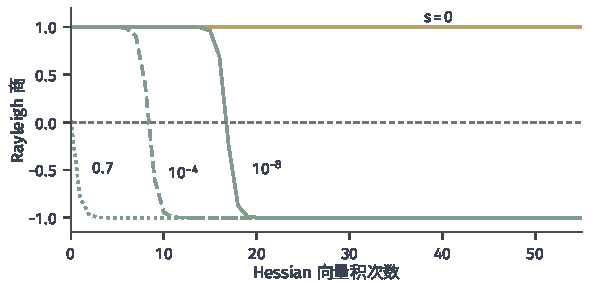
\includegraphics[width=100mm]{figures/05-optimization/02-smooth-optimization/matplotlib/saddle-krylov-blind/figure.pdf}
  \caption{$\bm{H}=\operatorname{diag}(-1,1)$，$L=2$，幂迭代的Rayleigh商随乘积次数的变化，起点是$(s,\sqrt{1-s^2})$。黄线$s=0$永远是$+1$，绿线从左到右$s=0.7,10^{-4},10^{-8}$，拐点依次右移，负曲率最终都被发现。}
  \label{fig:saddle-krylov-blind}
\end{BookInlineFigure}

\paragraph{找到和没有找到，结论不一样}
检测结束有两种结果，它们的可信程度差别很大。若$R^{(k)}\leq-\gamma$，这是一个算出来的事实：$\bm{v}$确实是曲率不超过$-\gamma$的方向，与随机抽样的运气无关。

若没有找到，结论就只能是概率性的。$\bm{v}^{(0)}$可能运气很差，迭代还没转过来就结束了。下面的定理说明，轮数足够多时，这种情况发生的概率很小。图~\ref{fig:saddle-detect-decision}概括了两种结论的区别。

\begin{BookInlineFigure}
  \centering
  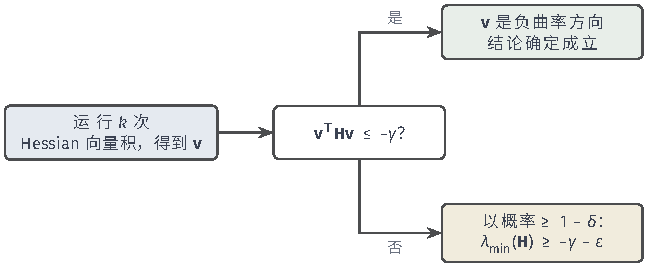
\includegraphics[width=109.6mm]{figures/05-optimization/02-smooth-optimization/tikz/saddle-detect-decision/figure.pdf}
  \caption{负曲率检测的两种结果。使用精确的Hessian向量积时，“找到”给出确定的结论；“未找到”只在随机起点成功的事件上成立，失败概率由$\delta$控制，$\varepsilon$是检测精度。}
  \label{fig:saddle-detect-decision}
\end{BookInlineFigure}

\begin{theorem}[幂迭代的概率保证]
 \label{thm:saddle-power}
 设$\bm{H}\in\mathbb{R}^{n\times n}$对称，$\lVert\bm{H}\rVert_2\leq L$，$\varepsilon\in(0,L]$，$\delta\in(0,1)$。$\bm{v}^{(0)}$在单位球面上均匀分布，幂迭代~\eqref{eq:saddle-power-iteration}运行$k$轮，其中
 \begin{equation}
  k\geq\frac{2L}{\varepsilon}\ln\frac{64Ln}{\pi\varepsilon\delta^3}.
  \label{eq:saddle-power-rounds}
 \end{equation}
 则至少以$1-\delta$的概率，
 \begin{equation}
  \bm{v}^{(k)\top}\bm{H}\bm{v}^{(k)}\leq\lambda_{\min}(\bm{H})+\varepsilon.
  \label{eq:saddle-power-guarantee}
 \end{equation}
\end{theorem}

\begin{proof}
 证明分两步：先说明随机起点在$\bm{q}_1$上的分量不会太小，再说明幂迭代把其余误差压下去。

 第一步处理起点。球面上的均匀分布可以写成$\bm{v}^{(0)}=\bm{z}/\lVert\bm{z}\rVert_2$，其中$\bm{z}$是标准正态向量。由旋转不变性，可以设$c_1=z_1/\lVert\bm{z}\rVert_2$是$\bm{v}^{(0)}$在$\bm{q}_1$上的分量。标准正态密度不超过$1/\sqrt{2\pi}$，所以
 \[
  \mathbb{P}\bigl(\lvert z_1\rvert\leq\tau\bigr)\leq\tau\sqrt{\frac{2}{\pi}}.
 \]

 取$\tau=\tfrac{\delta}{2}\sqrt{\pi/2}$，这个概率不超过$\delta/2$。又因为$\mathbb{E}\lVert\bm{z}\rVert_2^2=n$，由Markov不等式，
 \[
  \mathbb{P}\Bigl(\lVert\bm{z}\rVert_2^2>\frac{2n}{\delta}\Bigr)\leq\frac{\delta}{2}.
 \]

 因此至少以$1-\delta$的概率，两个事件都不发生，此时
 \[
  c_1^2\geq\frac{\tau^2}{2n/\delta}=\frac{\pi\delta^3}{16n}.
 \]

 第二步在这个事件上估计误差。记$a_i=L-\lambda_i$，$a_1$最大且$0\leq a_i\leq2L$；若$a_1=0$，$\bm{H}=L\bm{I}$，结论自动成立，下面设$a_1>0$。$\bm{v}^{(k)}$正比于$\bm{A}^k\bm{v}^{(0)}$，所以由$\bm{v}^\top\bm{H}\bm{v}=L-\bm{v}^\top\bm{A}\bm{v}$，
 \[
  \bm{v}^{(k)\top}\bm{H}\bm{v}^{(k)}-\lambda_{\min}
  =\frac{\sum_ic_i^2a_i^{2k}(a_1-a_i)}{\sum_ic_i^2a_i^{2k}}.
 \]

 把下标分成两组：$a_i\geq a_1-\varepsilon/2$的一组，分子中的因子$a_1-a_i$不超过$\varepsilon/2$，这一组对比值的贡献不超过$\varepsilon/2$。

 其余的下标满足$a_i<a_1-\varepsilon/2$，于是
 \[
  a_i^{2k}\leq a_1^{2k}\Bigl(1-\frac{\varepsilon}{2a_1}\Bigr)^{2k}
  \leq a_1^{2k}\exp\Bigl(-\frac{k\varepsilon}{a_1}\Bigr).
 \]

 分母至少是$c_1^2a_1^{2k}$，$a_1-a_i\leq a_1\leq2L$，$\sum_ic_i^2=1$，$a_1\leq2L$使指数不小于$k\varepsilon/(2L)$。所以这一组的贡献不超过
 \[
  \frac{2L}{c_1^2}\exp\Bigl(-\frac{k\varepsilon}{2L}\Bigr).
 \]

 代入$c_1^2$的下界和条件~\eqref{eq:saddle-power-rounds}，这个量不超过$\varepsilon/2$。两组相加，即得式~\eqref{eq:saddle-power-guarantee}。
\end{proof}

定理中各个量的作用可以逐项核对。$L/\varepsilon$来自幂迭代的收敛速度，要分辨相差$\varepsilon$的特征值，需要的轮数与$L/\varepsilon$成正比。$\ln n$和$\ln(1/\delta)$只出现在对数里，它们是随机起点要付的代价。

结论的含义是：运行满轮数仍然没有发现$R\leq-\gamma$时，以至少$1-\delta$的概率，
\begin{equation}
 \lambda_{\min}(\bm{H})\geq R^{(k)}-\varepsilon>-\gamma-\varepsilon.
 \label{eq:saddle-no-find}
\end{equation}

例中取$L=2$，$n=2$，$\varepsilon=\tfrac14$，$\delta=0.1$，式~\eqref{eq:saddle-power-rounds}要求$k\geq204$。上面的手算只用$2$次乘积就找到了方向。两者不矛盾：定理针对的是任意$\bm{H}$和最坏情形的起点分量，它要保证的是“没有找到”这个结论也能成立。

\paragraph{Lanczos方法}
幂迭代每轮只用最后一个向量，把前面的乘积结果都丢弃了。Lanczos方法保留整个Krylov子空间
\[
 \mathcal{K}_k=\operatorname{span}\bigl\{\bm{v}^{(0)},\bm{H}\bm{v}^{(0)},\ldots,\bm{H}^{k-1}\bm{v}^{(0)}\bigr\},
\]
并在这个子空间上取Rayleigh商的最小值。乘积次数相同，幂迭代的结果也落在同一个子空间内，所以Lanczos给出的值不会更差。它的三项递推和实现细节可参考\BookChapterRef{chap:krylov-methods}{卷二第15章“Krylov子空间法”}，这里只用它的结果：标准正交基下$\bm{H}$的投影是三对角矩阵$\bm{T}_k$，$\bm{T}_k$的最小特征值就是这个子空间上的最小Rayleigh商。

下面用一个三阶矩阵比较两者，它是在例子的Hessian上补一个中间特征值得到的：
\[
 \bm{H}=\operatorname{diag}(-1,1,2),\qquad
 \bm{v}^{(0)}=\frac{1}{\sqrt3}(1,1,1)^\top.
\]

第一步的对角元和残差是
\[
 \alpha_1=\frac23,\qquad
 \bm{w}=\bm{H}\bm{v}^{(0)}-\alpha_1\bm{v}^{(0)}
 =\frac{1}{3\sqrt3}\begin{bmatrix}-5\\1\\4\end{bmatrix},\qquad
 \beta_1=\lVert\bm{w}\rVert_2=\frac{\sqrt{14}}{3}.
\]

第二个基向量是$\bm{w}/\beta_1$，由此计算第二个对角元，得到
\[
 \alpha_2=\frac{-25+1+32}{42}=\frac{4}{21},\qquad
 \bm{T}_2=\begin{bmatrix}2/3&\sqrt{14}/3\\\sqrt{14}/3&4/21\end{bmatrix}.
\]

$\bm{T}_2$的最小特征值约为$-0.841$。同样用$2$次乘积，$L=2$的幂迭代$\bm{v}^{(1)}\propto(3,1,0)$给出$-0.8$。差距在小矩阵上不明显，在谱分布更不利时就很大了。

图~\ref{fig:saddle-power-lanczos}是一个$n=400$的例子。第二小的特征值紧贴最小特征值时，幂迭代几乎停滞，Lanczos仍然很快。原因是$k$次乘积相当于选一个$k$次多项式去放大$\bm{q}_1$分量，幂迭代固定用$a^k$，Lanczos等于在所有$k$次多项式中选最好的一个。

\begin{BookInlineFigure}
  \centering
  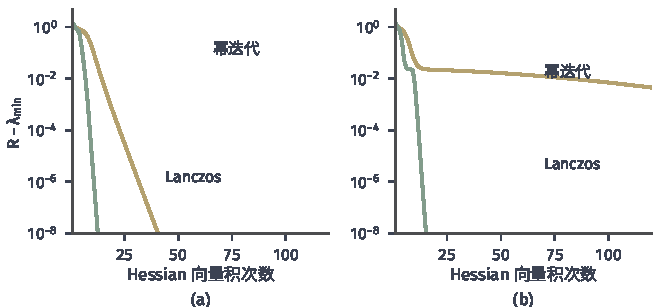
\includegraphics[width=112mm]{figures/05-optimization/02-smooth-optimization/matplotlib/saddle-power-lanczos/figure.pdf}
  \caption{同一个随机起点下幂迭代（黄，$L=2$）与Lanczos方法（绿）的Rayleigh商误差，$n=400$，$\lambda_{\min}=-0.2$，其余特征值在$[0.5,2]$上均匀取样，只有第二小的特征值另行指定。(a)第二小特征值为$0.3$。(b)第二小特征值为$-0.17$，与最小特征值很接近。}
  \label{fig:saddle-power-lanczos}
\end{BookInlineFigure}

定量结果是：均匀随机起点的Lanczos方法运行约$\sqrt{L/\varepsilon}\,\ln(n/\delta^2)$次乘积，就以至少$1-\delta$的概率达到精度$\varepsilon$。与定理~\ref{thm:saddle-power}相比，$L/\varepsilon$换成了它的平方根。证明需要用到Chebyshev多项式在区间外的增长估计，篇幅较长，读者可查阅数值线性代数的专门著作，这里只把它作为不加证明的事实使用。

Lanczos的计算也有代价：要存基向量才能算出方向，三项递推在有限精度下会失去正交性，运行次数多时需要重新正交化或重启。

\paragraph{误差怎样记入}
前面的结论默认Hessian向量积是精确的，用差分时要补上式~\eqref{eq:saddle-hvp-error}。对“找到”这一方，算出的$\hat{R}=\bm{v}^\top\hat{\bm{u}}$与真实Rayleigh商至多相差$Mh/2$，把判定条件改成$\hat{R}\leq-\gamma-Mh/2$，就能确定地推出$R(\bm{v})\leq-\gamma$。

对“没有找到”这一方，差分误差还会改变迭代本身，定理~\ref{thm:saddle-power}不能直接套用，分析时必须把每一轮的乘积误差累加进去。实际程序里，要做这一判断时通常用自动微分得到精确的乘积。表~\ref{tab:saddle-detect-compare}总结了几种方式。

\begin{BookInlineTable}
  \centering
  \begin{tabular}{@{}llll@{}}
    \toprule
    检测方式 & 成本 & 找到时 & 未找到时\\
    \midrule
    特征分解 & $O(n^3)$ & 确定 & 确定\\
    Cholesky试探 & $O(n^3)$，只判断 & 确定 & 确定\\
    幂迭代 & $O(\frac{L}{\varepsilon}\ln\frac{n}{\delta})$次乘积 & 确定 & $\geq1-\delta$\\
    Lanczos & $O(\sqrt{\frac{L}{\varepsilon}}\ln\frac{n}{\delta})$次乘积 & 确定 & $\geq1-\delta$\\
    差分乘积 & 每次两个梯度 & 加余量$Mh/2$ & 累加误差\\
    \bottomrule
  \end{tabular}
  \caption{负曲率检测方式的比较，“确定”不计舍入误差，“$\geq1-\delta$”指结论成立的概率。$O(\cdot)$中省略了$L/\varepsilon$的对数因子。}
  \label{tab:saddle-detect-compare}
\end{BookInlineTable}

